% !TeX spellcheck = en_US

\chapter{Practical Challenges}\label{chp:practical_challenges}

\section{Training data}
There are two options when selecting a data set that can be used to train the neural networks. Either an already available data set is used, whether on a paid or free basis, or a new data set is created. Currently, machine learning and deep learning are popular topics, especially deep learning. As a result, more data sets are available publicly and at no cost, especially in the area of image processing – such as segmentation, facial recognition, and object detection. Free data sets consisting of aerial imagery are provided by several sources (\cite{VolodymyrMnih.2013}, \cite{spacenet}, \cite{isprs-vaihingen}, \cite{isprs-potsdam}, \cite{Helber.20170831}, \cite{deepsat}).
Despite this availability of data sets, we decided to make our own. The data set would consist solely of open data, using Microsoft Bing for the imagery and OpenStreetMap for the vector data. Due to this, a tool named Airtiler \cite{airtiler} was developed and is described in detail in \autoref{chp:theoretical_and_experimental_results}.

It can be assumed that in the future, more Swiss cantons\footnote{Switzerland consists of 26 cantons, which form the Swiss Confederation} will make high-resolution orthophotos publicly available. At the time of writing, the canton of Zurich played a pioneering role and made several of its data sources publicly and freely available\footnote{https://geolion.zh.ch/ (15.06.18)}. However, at the time of this writing it was not an option to use these images for our work because it would have been a rather small data set.


\section{Prediction accuracy}

\subsection{Class probability}
After the first training of the neural network, the results were not quite as good as expected. Although most of the buildings were predicted as buildings, other classes – like tennis courts – were also predicted as buildings. The network was therefore retrained using the additional and incorrectly determined classes (like tennis courts). However, instead of the distinction between buildings and tennis courts becoming more accurate, the overall prediction accuracy was even worse. This might have been the result of the network having to solve a more complex task, by deciding which class an object belonged to, instead of a simple yes-no decision. In addition, the training data were highly imbalanced as the images contained many more buildings than tennis courts.

A solution could be to train the network separately several times to obtain several models, each trained for a specific class. Another solution could be to weight the loss according to the relative amount of the specific class, based on the size of the whole data set.

\subsection{Outline}
\autoref{fig:challenges:small_predictions} shows that the predictions were generally rather too small, compared to the corresponding orthophoto. This might have been the result of slightly misaligned masks, since the masks and the images were generated separately.

\begin{figure}[H]
    \centering
	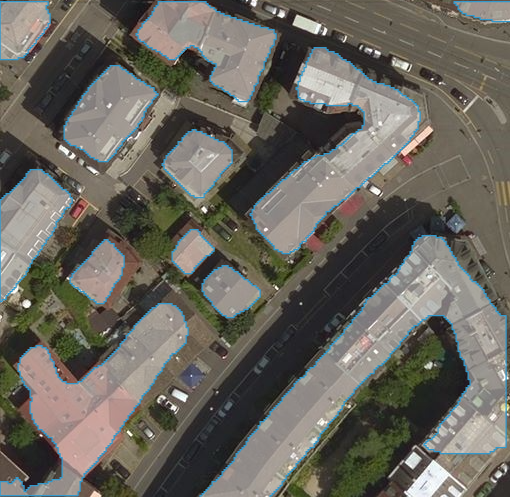
\includegraphics[width=0.4\linewidth]{chapters/challenges/images/small_predictions.png}
	\caption{Too small predictions}
	\label{fig:challenges:small_predictions}
\end{figure}


\section{Regularization of building outlines}
Once a network has been trained, it can be used to make predictions on images it has never "seen" before. However, in certain situations the predictions are far from perfect, especially if the building is partially covered by trees or has unclear outlines. Examples are shown in \autoref{fig:challenges:building_masks}. The predictions in such cases are mere approximations of the actual ground truths.

\begin{figure}[H]
	\centering
	\begin{subfigure}{0.4\textwidth}
    	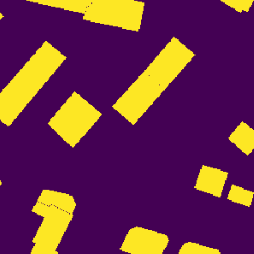
\includegraphics[width=0.9\linewidth]{chapters/challenges/images/predicted_masks_gt.png}		    \caption{Actual ground truth}
    	\label{fig:challenges:predicted_building_masks_gt}
	\end{subfigure}~
		\begin{subfigure}{0.4\textwidth}
    	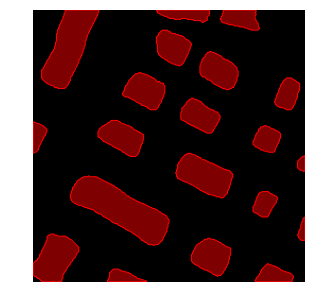
\includegraphics[width=0.9\linewidth]{chapters/challenges/images/predicted_masks.png}		    \caption{Predicted building masks}
    	\label{fig:challenges:predicted_building_masks}
	\end{subfigure}
	\caption{Predicted masks and actual ground truth}
	\label{fig:challenges:building_masks}
\end{figure}

Because of the inaccuracies in predicted building masks, the contours of such predictions cannot directly be used to create the vectorized outlines. Instead, the predictions must be regularized. The approach we used is shown in \autoref{fig:challenges:rectangularization} and was similar to that described in literature \cite{Partovi.2017}. The single steps are described in detail in the following sections.

\begin{figure}[H]
\centering
\begin{tikzpicture}[node distance = 2cm, auto, scale=0.7, every node/.style={transform shape}]
    % Place nodes
    \node [cloud] (mask) {Predicted mask};
    \node [block, below of=mask] (extract_contour) {Extract contour};
    \node [cloud, below of=extract_contour] (contour) {Approximated contour};
    \node [block, below of=contour] (segment) {Line segmentation};
    \node [cloud, below of=segment] (line_segments) {Line segments};
    \node [block, below of=line_segments] (assign_orientation) {Create orientation classes};
    \node [block, below of=assign_orientation] (assign_neighborhoods) {Create neighborhoods};
    \node [block, below of=assign_neighborhoods] (rotate_lines) {Rotate lines};
    \node [block, below of=rotate_lines] (gap_filling) {Gap filling};
    \node [cloud, below of=gap_filling] (corner_points) {Building corner points};

    % Draw edges
    \path [line,dashed] (mask) -- (extract_contour);
    \path [line,dashed] (extract_contour) -- (contour);
    \path [line,dashed] (contour) -- (segment);
    \path [line,dashed] (segment) -- (line_segments);
    \path [line,dashed] (line_segments) -- (assign_orientation);
    \path [line] (assign_orientation) -- (assign_neighborhoods);
    \path [line] (assign_neighborhoods) -- (rotate_lines);
    \path [line] (rotate_lines) -- (gap_filling);
    \path [line,dashed] (gap_filling) -- (corner_points);
\end{tikzpicture}
	\caption{Rectangularization procedure}
	\label{fig:challenges:rectangularization}
\end{figure}

\subsection{Contour extraction}
The first step of the building outline regularization procedure consists of obtaining the contour from the predicted mask, which covers the whole building. The extraction is performed using the marching squares algorithm \cite{Maple.2003}. In this algorithm, a square consisting of four cells is moved (marched) along the contour in such a way that at least one cell always covers the object to be contoured. Additionally, the square always has a state that is derived from the content of its cells, according to \eqref{equ:challenges:marching_squares_state}. The cells are traversed in counter-clockwise order.

\newenvironment{conditions}
  {\par\vspace{\abovedisplayskip}\noindent\begin{tabular}{>{$}l<{$} @{${}={}$} l}}
  {\end{tabular}\par\vspace{\belowdisplayskip}}

\begin{equation}
\begin{split}
	s	&= \displaystyle\sum_{i=0}^3 2^i f(c_i) \\
		&= 2^0 * f(c_0) + 2^1 * f(c_1) + 2^2 * f(c_2) + 2^3 * f(c_3) \\
		&= f(c_{bottomLeft}) + 2 * f(c_{bottomRight}) + 4 * f(c_{topRight}) + 8 * f(c_{topLeft})
	\label{equ:challenges:marching_squares_state}
\end{split}
\end{equation}
where:
\begin{itemize}[label=]
    \item $c_i$: The value of the cell $i$
    \item $c_0$: The bottom left cell
\end{itemize}

and

\[ f(c_i) =
  \begin{cases}
    0  & \text{if $c_i \leq 0$}\\
    1  & \text{if $c_i > 0$}
  \end{cases}
\]

After the contour has been extracted, its number of points is reduced using a Douglas-Peucker algorithm \cite{Douglas.1973}. The reason for this is that the contour has pixel accuracy. That means there may be several points on the same horizontal or vertical line, although the startpoint and endpoint of each line would be enough to represent the line. In addition, the fewer the points that are represented on a contour, the faster the processing will be.

\begin{figure}[H]
    \centering
	\begin{subfigure}{0.45\textwidth}
    	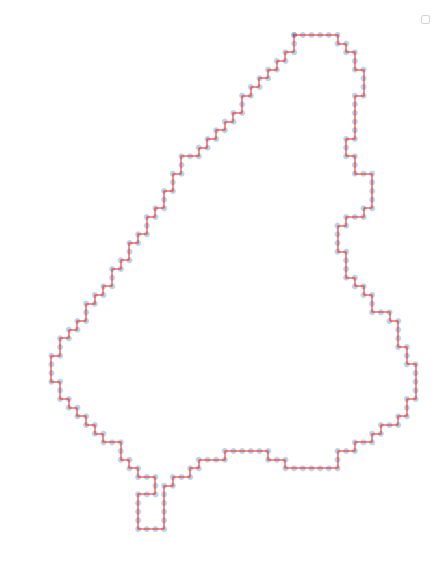
\includegraphics[width=0.9\linewidth]{chapters/challenges/images/original_contour.png}		    	\caption{Original contour}
	\end{subfigure}~
	\begin{subfigure}{0.45\textwidth}
    	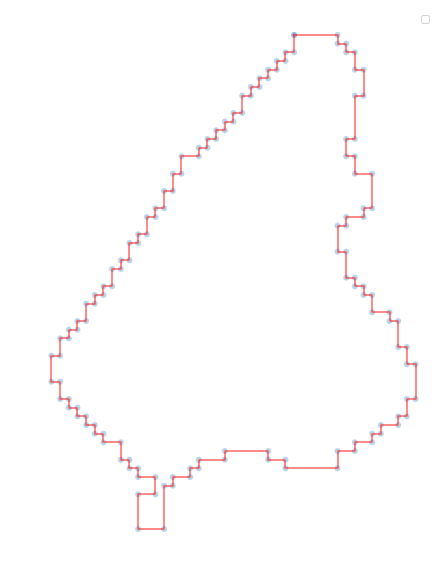
\includegraphics[width=0.9\linewidth]{chapters/challenges/images/approx_contour.png}       			\caption{Approximated contour}
	\end{subfigure}
	\caption{Contour before and after approximation. It can be seen, that the contour on the right consists of much lesser points.}
	\label{fig:challenges:contour_approximation}
\end{figure}


\subsection{Line segmentation}
Once the contour has been extracted, it is split into many line segments. To do so, the main direction of the building is determined using the Hough Transformation \cite{Duda.1972}. The result of the Hough Transformation is a data-structure which contains an angle, a distance and a number. The combination of the angle and the distance, from a predefined reference point, leads to a line. The number is the number of points which lie on the constructed line. This algorithm can be used to detect the main building orientation, that is, the longest contour-line of any orientation. The angle of the line that is found is called the main building orientation.

Once the main building orientation is known, the line segmentation starts at the point which has the smallest distance from the line. The whole procedure is depicted in \autoref{alg:challenges:line_segmentation}.

\begin{algorithm}[H]
\KwData{Contour points, startpoint}
\KwResult{Lines}
rearrange points so that startpoint == points[0]\\
lines = []\\
\While{any points left}{
	segment = remove first 3 elements from points\\
	\While{points is not empty}{
		p = points.first()\\
		err = root mean square error of distance between segment.last() and p\\
		\If{err > threshold}{
			break
		}
		segment.append(p)\\
		points.remove(p)\\
	}
	\If{segment.length() >= 3}{
		line = fit line to points of segment\\
		lines.append(line)
	}
}
\caption{Line segmentation}
\label{alg:challenges:line_segmentation}
\end{algorithm}

\subsection{Create orientation classes}
After the line segmentation, an orientation is assigned to each line. Generally, most buildings consist of mainly right angles, although some buildings do exist for which this assumption is untrue. Hence, orthogonality is preferred but other angles remain possible. Algorithm~\ref{alg:challenges:define_orientations} shows the procedure which assigns a main orientation class to each line, and defines the line’s nature in terms of it being parallel or orthogonal to the longest line in the same orientation class.

\begin{figure}[H]
    \centering
	\begin{subfigure}{0.4\textwidth}
    	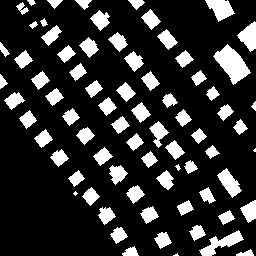
\includegraphics[width=0.9\linewidth]{chapters/challenges/images/regular_building_masks.png}		    \caption{Regular buildings}
    	\label{fig:challenges:regular_buildings}
	\end{subfigure}~
	\begin{subfigure}{0.4\textwidth}
    	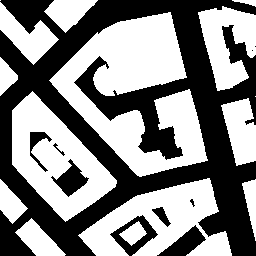
\includegraphics[width=0.9\linewidth]{chapters/challenges/images/irregular_building_masks.png}       	\caption{Non-orthogonal buildings}
    	\label{fig:challenges:irregular_buildings}
	\end{subfigure}
	\caption{Various building types with regard to corner angles}
	\label{fig:challenges:building_ground_truths}
\end{figure}

\begin{algorithm}[H]
\KwData{Lines, angleThreshold}
	\While{any line without orientation}{
		line = longest of unprocessed lines\\
		line.orientation = angle between line and horizontal-line \\
		\ForEach{line li without orientation}{
			a = angle between line and li\\
			\If{a $\leq$ angleThreshold}{
				li.orientation = line.orientation
				li.orthogonal = line.orthogonalTo(line)
			}
		}
	}
\caption{Orientation assignment}
\label{alg:challenges:define_orientations} 
\end{algorithm}

\subsection{Create neighborhoods}
At this point, each line segment belongs to an orientation class, and the parallelity or orthogonality of each line to the orientation class’s main line is known. However, the spatial location of each line has not been considered yet and this must be performed in the current step. Clusters of neighboring lines are created within each orientation class. These clusters make it possible to identify lines which may be better placed in another orientation class. The assumption underlying this step is that it is unlikely for a line $k$ of the orientation class $x$ to be surrounded by lines of the orientation class $y$. In this case, line $k$ will be assigned to orientation class $y$.

\subsection{Update line orientation}
Finally, the lines are adjusted to their orientation class with regard to each line’s parallelity or orthogonality. The result of such an adjustment is shown in \autoref{fig:challenges:adjusted_lines}. The figure illustrates a single orientation of class and lines, which have been adjusted either parallel or orthogonal to the orientation class. To create the final building outline, all that remains is to fill in the gaps between line segments.

\begin{figure}[H]
    \centering
	\begin{subfigure}{0.45\textwidth}
    	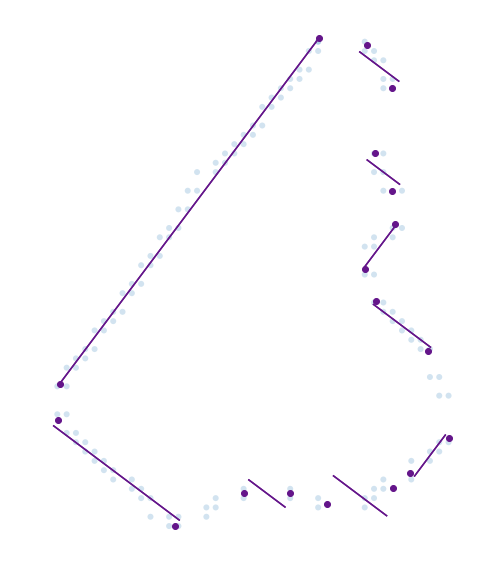
\includegraphics[width=0.9\linewidth]{chapters/challenges/images/adjusted_lines.png}		    		\caption{Adjusted lines}
    	\label{fig:challenges:adjusted_lines}
	\end{subfigure}~
	\begin{subfigure}{0.45\textwidth}
    	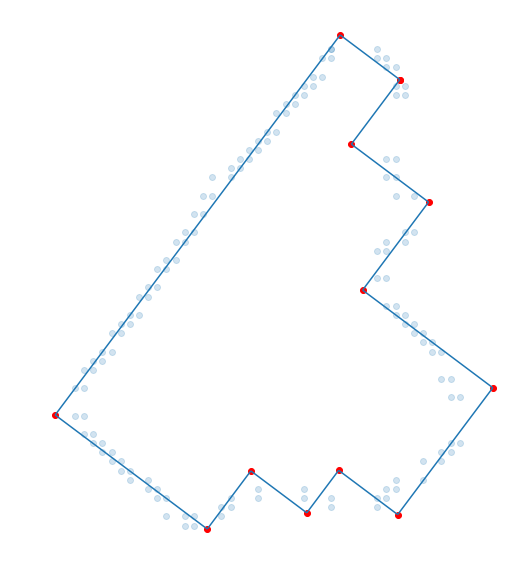
\includegraphics[width=0.9\linewidth]{chapters/challenges/images/filled_gaps.png}       				\caption{Final building outline}
    	\label{fig:challenges:final_building_outline}
	\end{subfigure}
	\caption{Building outline. Left panel: adjusted lines; right panel: final outline with gaps filled in.}
	\label{fig:challenges:building_ground_truths}
\end{figure}